\documentclass[11pt,a4paper]{article}
\usepackage[utf8]{inputenc}
\usepackage[margin=1.6cm]{geometry}
\usepackage{graphicx}
\usepackage{xcolor}
\usepackage{tabularx}
\usepackage{booktabs}
\usepackage{enumitem}

\definecolor{navy}{HTML}{060C1A}
\definecolor{gold}{HTML}{C5A059}
\definecolor{primary}{HTML}{0284C7}
\definecolor{dark}{HTML}{0F172A}

\pagestyle{plain}

\begin{document}

% ============================================================
% TRANG BIA
% ============================================================
\begin{center}
    \vspace*{0.6cm}
    {\Huge\bfseries\color{navy} DAU TRUONG OLYMQUIZ ARENA}\\[0.3cm]
    {\LARGE\bfseries\color{primary} CAM NANG VAN HANH TOAN DIEN VA CHI TIET}\\[0.3cm]
    {\large\bfseries\color{gold} Huong Dan Tung Man Hinh -- Day Du 13 Anh Chup Thuc Te -- De Hieu 100\%}\\[0.2cm]
    \rule{\textwidth}{1.5pt}
    \vspace{0.3cm}
    {\small Tai lieu danh cho Ban Giam Khao, Thu Ky Tran Dau va 4 Thi Sinh}
    \vspace{0.5cm}
\end{center}

\noindent\textbf{\large QUY TRINH VAN HANH 3 BUOC NHANH:}\\
\begin{enumerate}[leftmargin=*,itemsep=3pt]
    \item \textbf{Truoc tran dau}: Mo \texttt{/admin/players} $\rightarrow$ Copy link va ma PIN gui cho 4 ban thi sinh.
    \item \textbf{Trong tran dau}: Mo \texttt{/admin/live} $\rightarrow$ Nhan phim \textbf{Space} (Dem gio) $\rightarrow$ Bam \textbf{Mo Dap An} $\rightarrow$ Nhan phim \textbf{G} (Cham diem tu dong).
    \item \textbf{Ket thuc tran}: Bam nut \textbf{[4. Bang Vang Trao Giai]} tren Ban Giam Khao de may chieu vinh danh Quan quan!
\end{enumerate}

\vspace{0.3cm}
\hrule
\vspace{0.5cm}

% ============================================================
% MAN HINH 1: QUAN LY THI SINH & CAP MA PIN
% ============================================================
\noindent{\Large\bfseries\color{primary} MAN HINH 1: QUAN LY 4 THI SINH VA CAP MA PIN}\\[0.1cm]
\noindent\textit{Duong dan: \texttt{/admin/players} | Nguoi thuc hien: Ban To Chuc / Giam Khao}\\[0.2cm]
\textbf{Muc dich}: Buoc chuan bi quan trong nhat truoc khi tran dau dien ra.
\begin{itemize}[leftmargin=*,noitemsep]
    \item \textbf{Nut [SAO CHEP LINK THI DAU]}: Bam de copy link phong thi kem ma PIN rieng cua tung may gui cho thi sinh qua Zalo/Facebook.
    \item \textbf{O Ma PIN (1111, 2222, 3333, 4444)}: Ma bao mat rieng cua tung buc may, ngan chan nguoi ngoai vao nham phong thi.
    \item \textbf{Bo 3 Nut Reset Tong (Goc phai tren)}:
    \begin{itemize}
        \item \textbf{[Reset Diem Ve 0]}: Dua diem cua ca 4 thi sinh ve so 0 truoc tran.
        \item \textbf{[Tao Moi 4 Ma PIN]}: Cap 4 ma PIN ngau nhien moi va huy bo ma cu.
        \item \textbf{[Reset Ca 4 Buc May]}: Xoa trang toan bo thong tin san sang cho tran moi.
    \end{itemize}
\end{itemize}

\begin{center}
    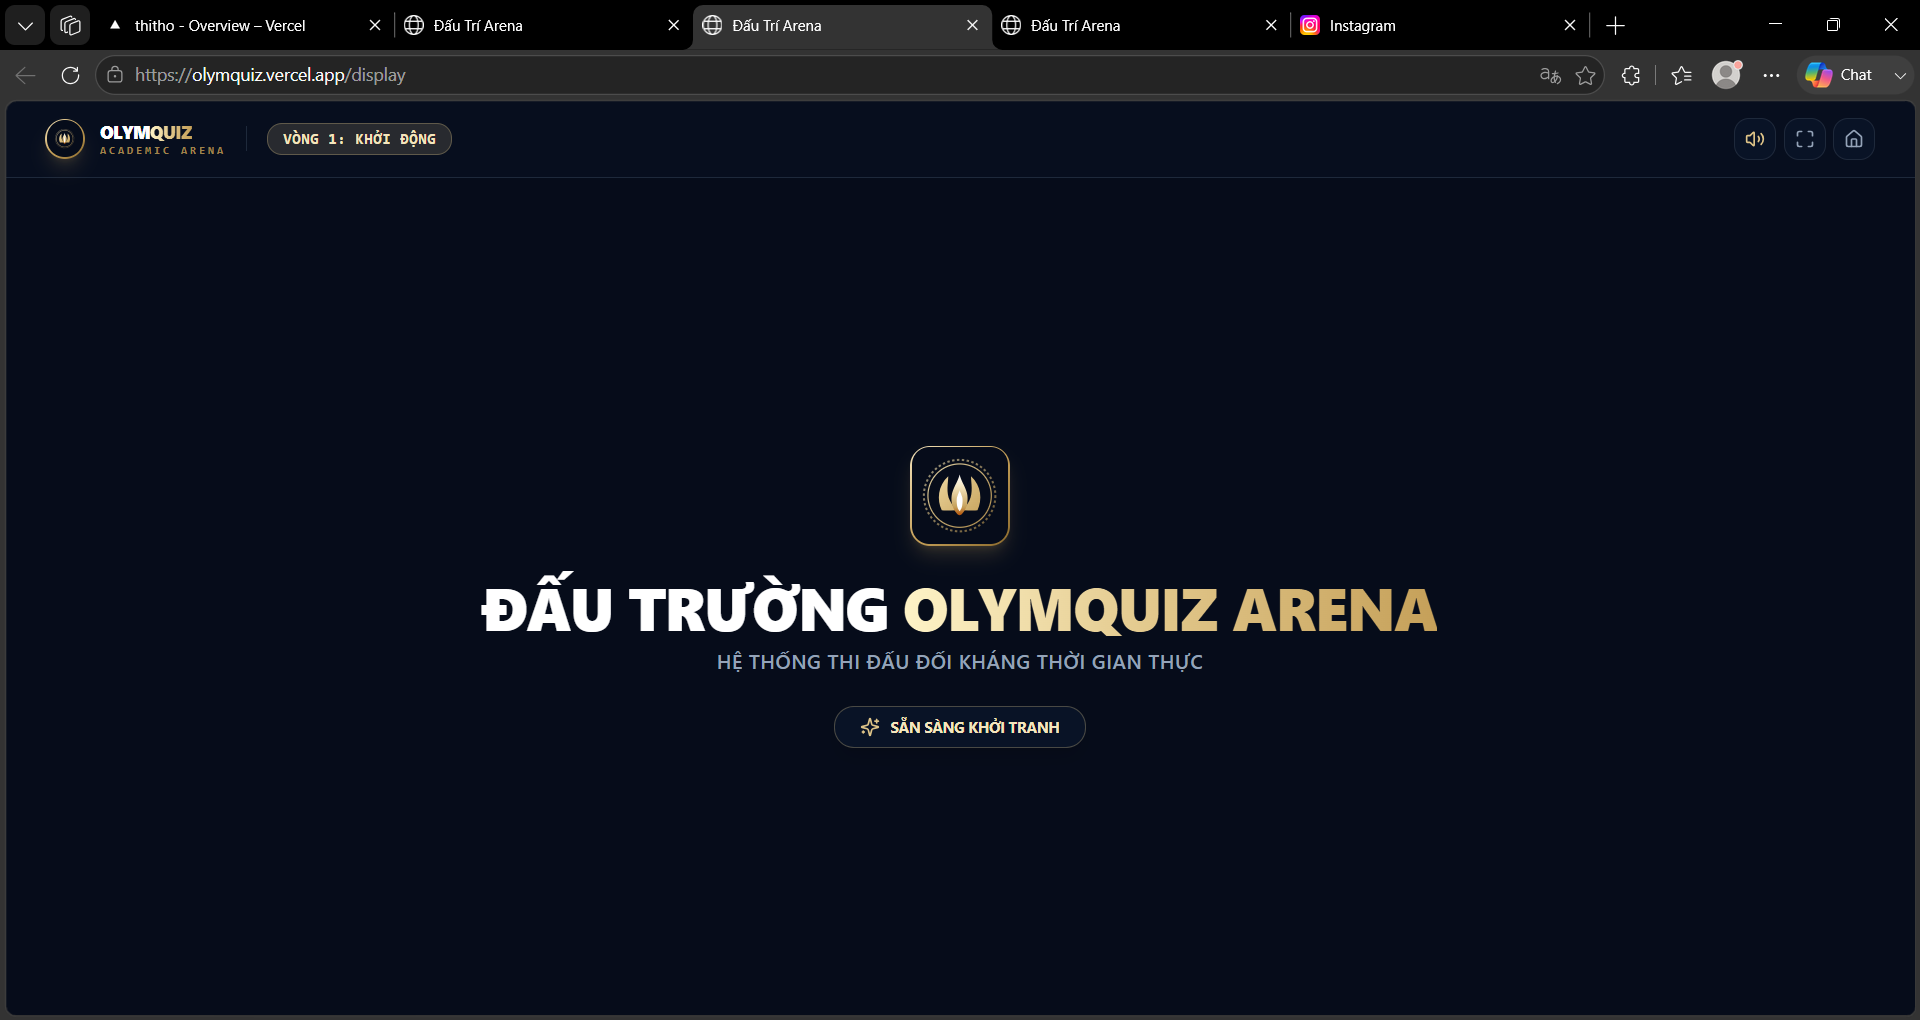
\includegraphics[width=0.95\textwidth]{screenshots/12_admin_players.png}
\end{center}

\newpage

% ============================================================
% MAN HINH 2: THI SINH NHAP PIN
% ============================================================
\noindent{\Large\bfseries\color{primary} MAN HINH 2: THI SINH NHAP MA PIN VAO PHONG THI}\\[0.1cm]
\noindent\textit{Duong dan: \texttt{/player/1} den \texttt{/player/4} | Nguoi thuc hien: Thi Sinh}\\[0.2cm]
\textbf{Muc dich}: Giup thi sinh dang nhap an toan vao dung vi tri may cua minh.
\begin{itemize}[leftmargin=*,noitemsep]
    \item Thi sinh mo link do Ban To Chuc gui tren dien thoai hoac laptop.
    \item Go ma PIN 4 chu so do Giam Khao cap $\rightarrow$ Bam nut \textbf{[XAC NHAN VAO PHONG THI]}.
    \item Sau khi dang nhap thanh cong, buc may se ket noi truc tiep voi he thong thi dau.
\end{itemize}

\begin{center}
    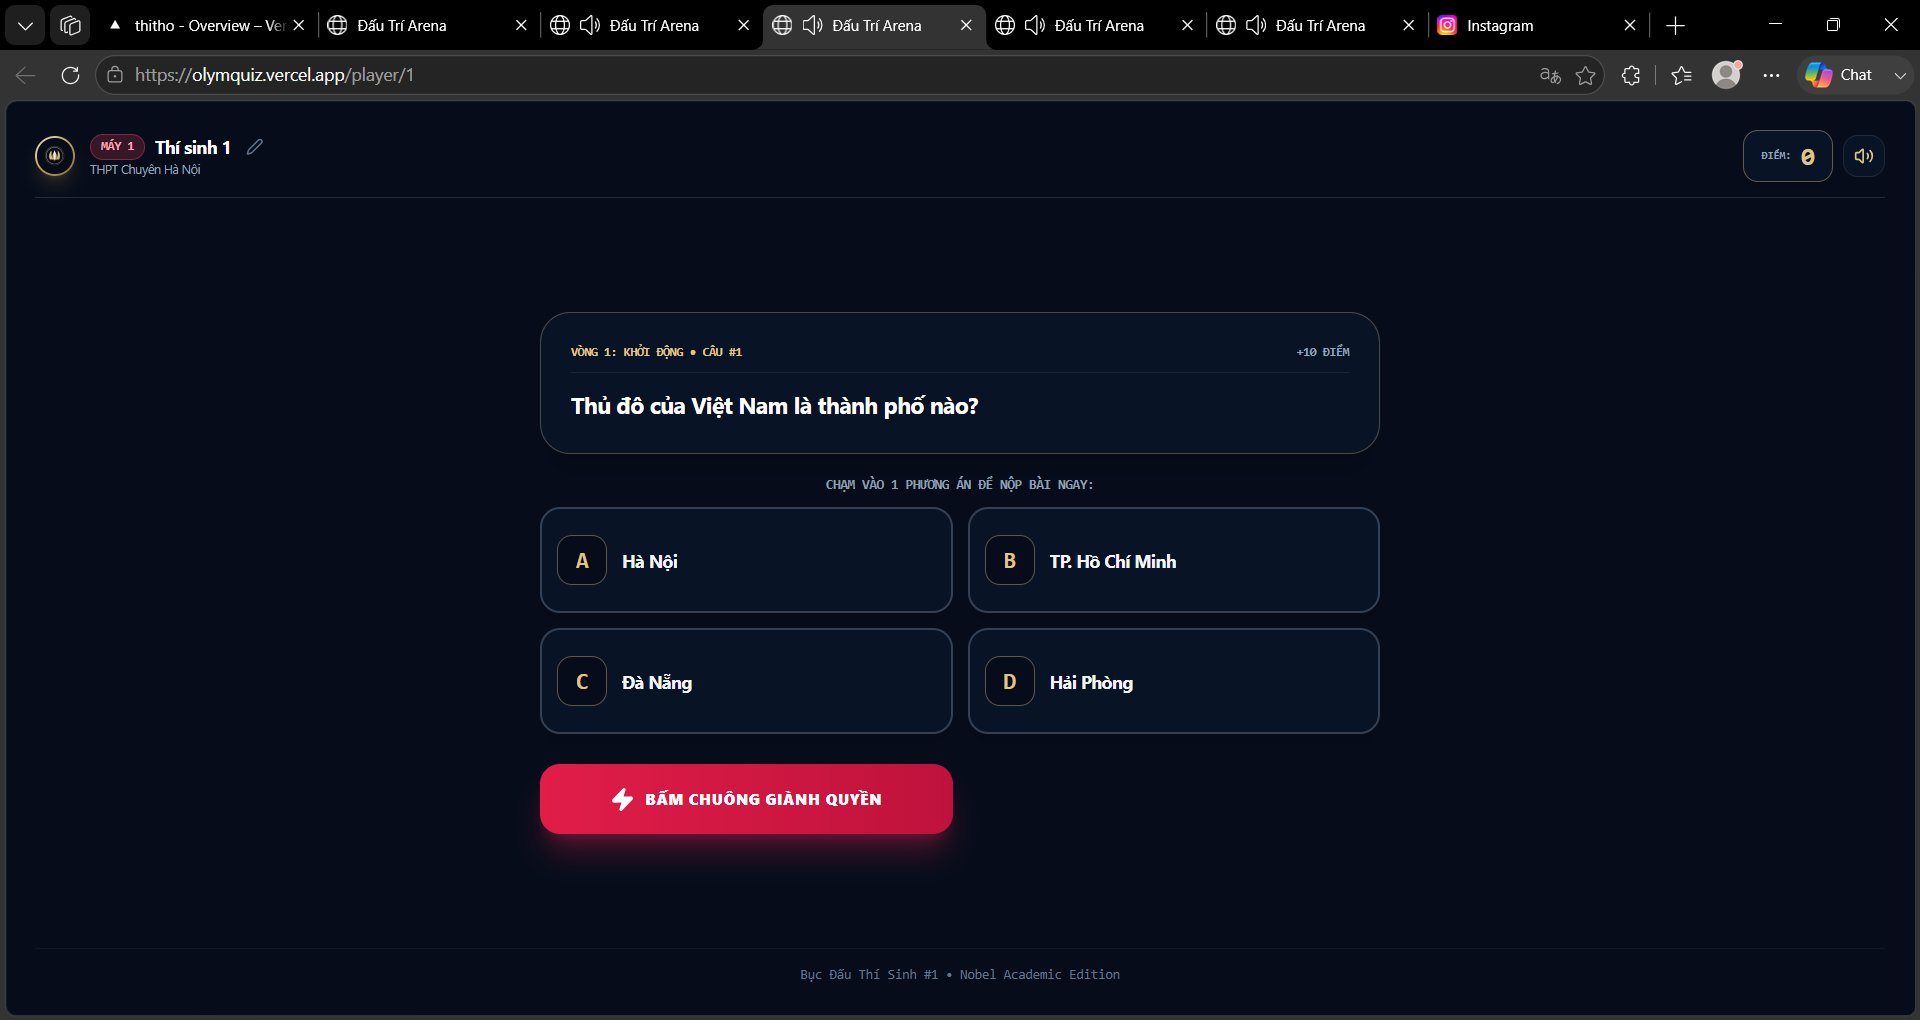
\includegraphics[width=0.95\textwidth]{screenshots/01_login_pin.png}
\end{center}

\vspace{0.4cm}

% ============================================================
% MAN HINH 3: BUC THI SINH THI DAU
% ============================================================
\noindent{\Large\bfseries\color{primary} MAN HINH 3: GIAO DIEN THI DAU TRUC TIEP CUA THI SINH}\\[0.1cm]
\noindent\textit{Duong dan: \texttt{/player/[slot]} | Nguoi thuc hien: Thi Sinh}\\[0.2cm]
\textbf{Muc dich}: Noi thi sinh doc de bai va nop cau tra loi trong suot tran dau.
\begin{itemize}[leftmargin=*,noitemsep]
    \item \textbf{4 The Trac Nghiem To (A, B, C, D)}: Thi sinh chi can \textbf{cham 1 lan vao o dap an}. Man hinh se doi sang mau xanh ngoc xac nhan nop bai thanh cong kem so giay nop.
    \item \textbf{Tu Luan va O Chu (Vong 2)}: Go chu vao o nhap va bam nut \textbf{[Nop Bai]}.
    \item \textbf{Bam Chuong Cuop Diem (Vong 4)}: Nut chuong do to se sang len khi co cau cuop diem, ai bam nhanh nhat se gianh quyen tra loi.
\end{itemize}

\begin{center}
    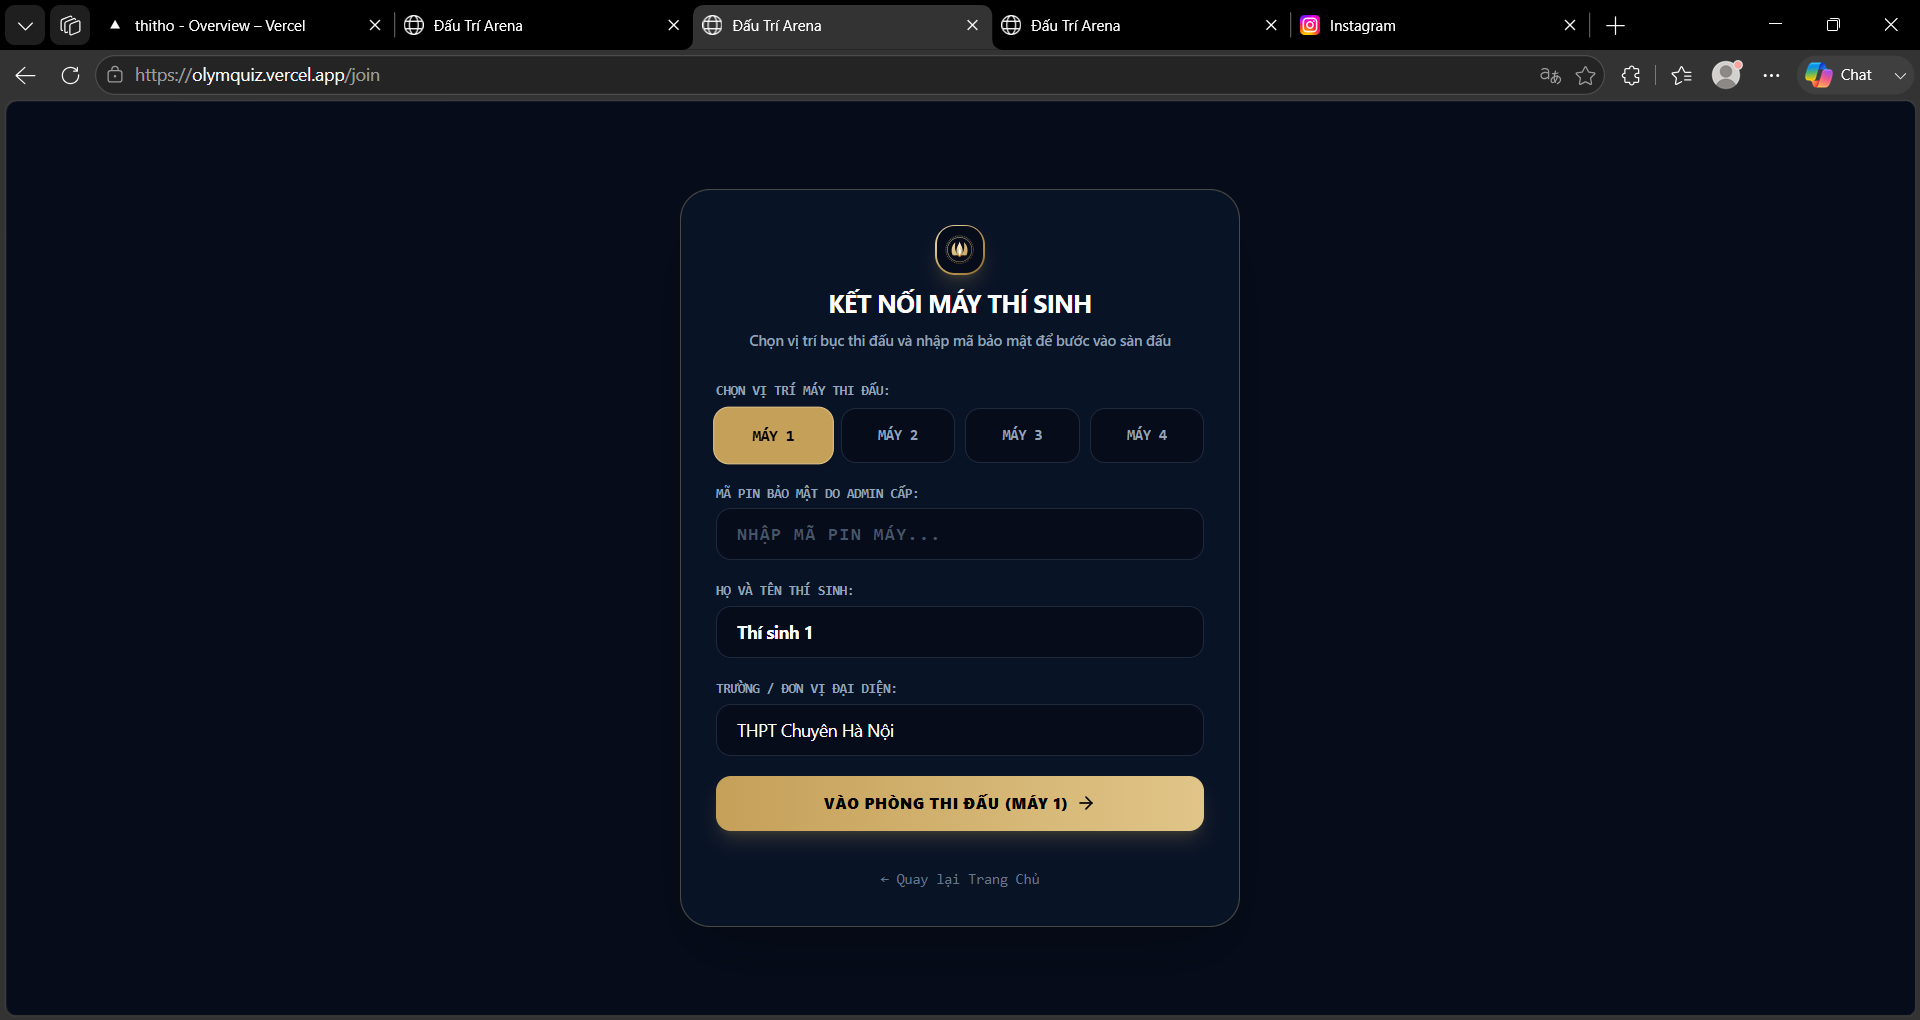
\includegraphics[width=0.95\textwidth]{screenshots/11_player_screen.png}
\end{center}

\newpage

% ============================================================
% MAN HINH 4: BAN GIAM KHAO LIVE
% ============================================================
\noindent{\Large\bfseries\color{primary} MAN HINH 4: BAN DIEU HANH BAN GIAM KHAO LIVE}\\[0.1cm]
\noindent\textit{Duong dan: \texttt{/admin/live} | Nguoi thuc hien: Ban Giam Khao / Thu Ky}\\[0.2cm]
\textbf{Muc dich}: Trung tam dieu phoi nhip do, tinh gio va cham diem tran dau.
\begin{itemize}[leftmargin=*,noitemsep]
    \item \textbf{Thanh Chon 5 Slide (Hang tren cung)}: 1-Click doi man may chieu sang: \textbf{Cau hoi}, \textbf{Gioi thieu}, \textbf{The le 4 vong}, \textbf{Bang vang}, \textbf{Standby}.
    \item \textbf{Dong Ho Master Timer (Cot trai)}: Bam phim \textbf{Space} de Bat dau/Tam dung. Phim \textbf{R} de Reset. Nut \textbf{15s, 20s, 30s} de chinh nhanh thoi gian.
    \item \textbf{Chon Vong va Cau Hoi (Cot trai duoi)}: Chon Vong 1, 2, 3, 4 va cau hoi \#1, \#2, \#3...
    \item \textbf{Bo 3 Nut Dieu Phoi (Khung giua)}:
    \begin{itemize}
        \item \textbf{Khoa Nop (Phim L)}: Khoa buc khong cho thi sinh nop hoac sua dap an nua.
        \item \textbf{Mo Dap An}: Chieu dap an dung len may chieu va buc thi sinh.
        \item \textbf{Cham Diem (Phim G)}: Tu dong so khop dung/sai va cong diem tuc thi vao bang tong.
    \end{itemize}
    \item \textbf{Cot Giam Sat 4 Thi Sinh (Cot phai)}: Xem cau tra loi va so giay cua tung ban. Co cac nut \textbf{+20, +30, -10} de cong hoac tru diem thu cong.
\end{itemize}

\begin{center}
    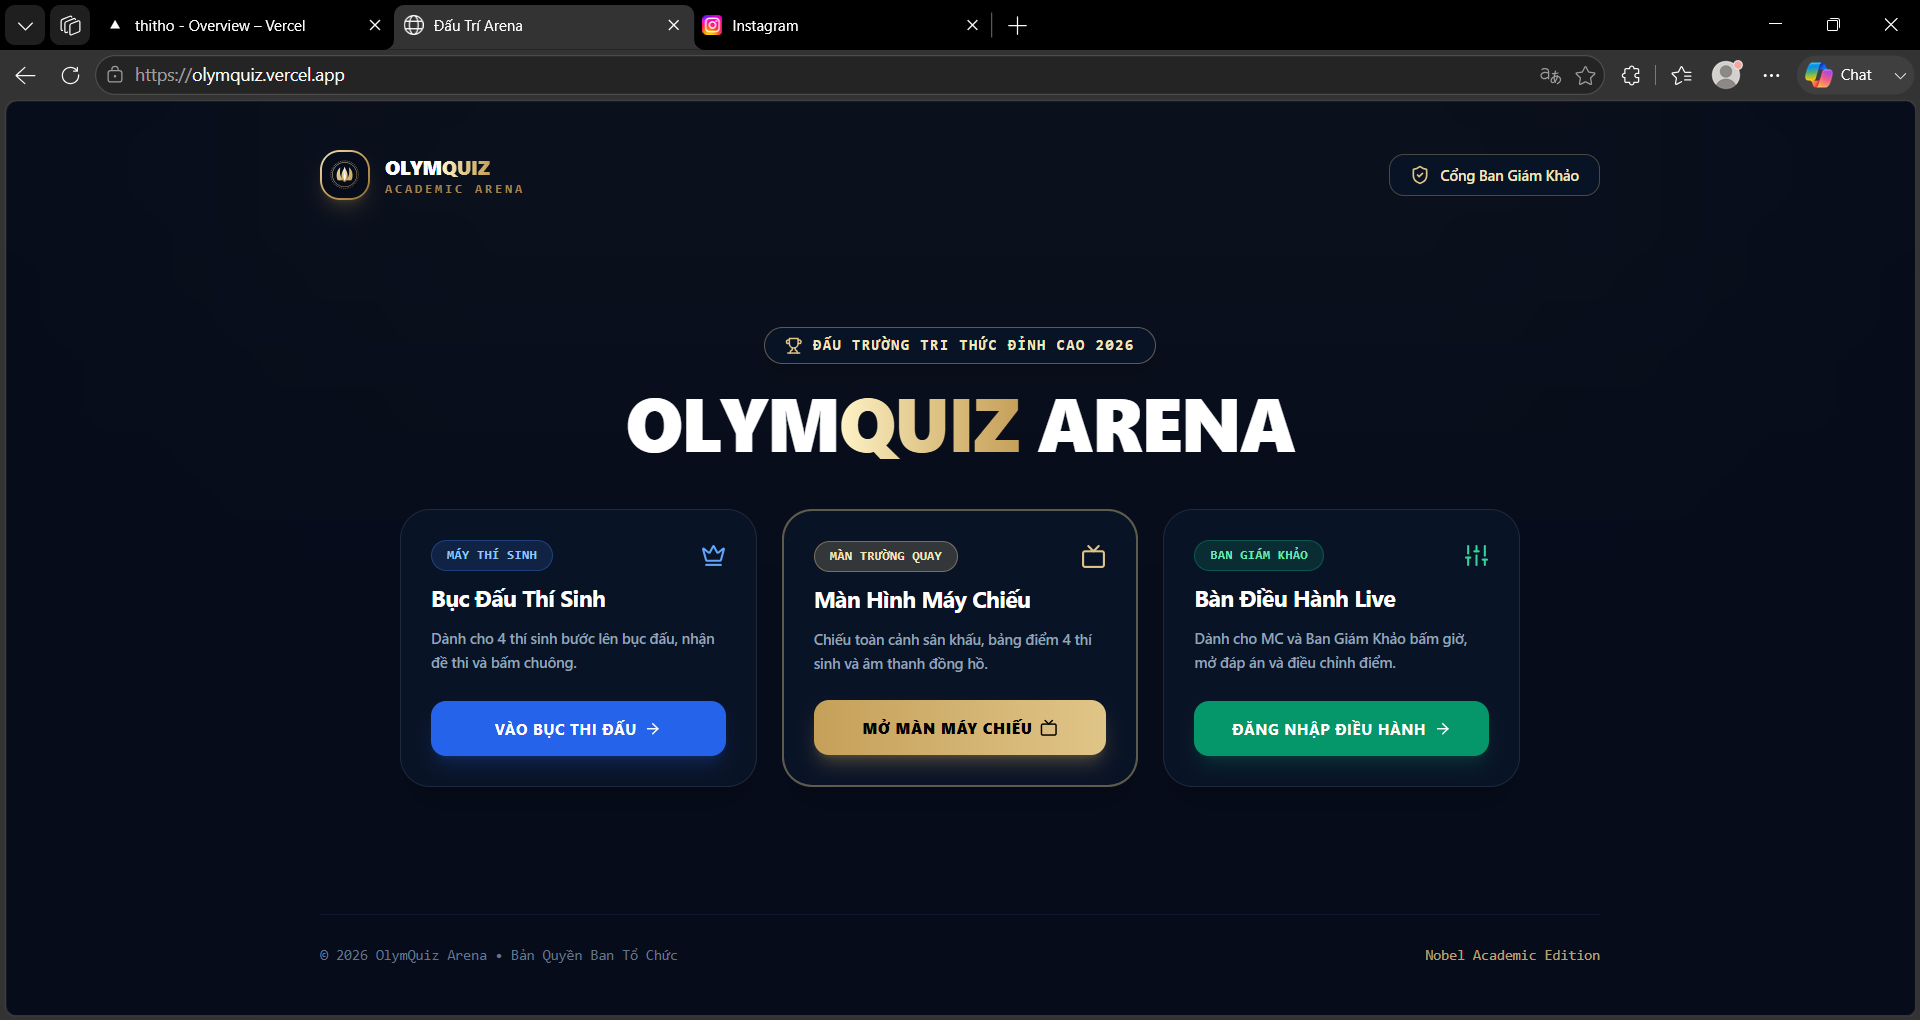
\includegraphics[width=0.95\textwidth]{screenshots/13_admin_live.png}
\end{center}

\vspace{0.2cm}
\noindent\textbf{Bang Phim Tat Tien Loi Cho Giam Khao:}\\
\begin{tabularx}{\textwidth}{l l X}
\toprule
\textbf{Phim Tat} & \textbf{Chuc Nang} & \textbf{Hanh Dong Nhanh} \\
\midrule
\textbf{Space} & Bat Dau / Tam Dung & Chay hoac dung dem nguoc thoi gian cau hoi. \\
\textbf{L} & Khoa Nop Bai & Khoa khong cho 4 thi sinh nop bai nua. \\
\textbf{G} & Cham Diem & Tu dong kiem tra dung/sai va cong diem tuc thi. \\
\textbf{R} & Reset Dong Ho & Tra thoi gian ve ban dau va xoa bai nop cu cua cau. \\
\bottomrule
\end{tabularx}

\newpage

% ============================================================
% MAN HINH 5: SLIDE GIOI THIEU THI SINH
% ============================================================
\noindent{\Large\bfseries\color{primary} MAN HINH 5: SLIDE GIOI THIEU 4 THI SINH XUAT SAC}\\[0.1cm]
\noindent\textit{Man hinh May Chieu Hoi Truong (\texttt{/display})}\\[0.2cm]
\textbf{Muc dich}: Chieu toan canh 4 Card thi sinh trang trong truoc tran dau de MC gioi thieu tung ban buoc len san khau.
\begin{itemize}[leftmargin=*,noitemsep]
    \item Hien thi so may (MAY 1, 2, 3, 4), Ho ten, Don vi dai dien va diem so khoi dau.
\end{itemize}

\begin{center}
    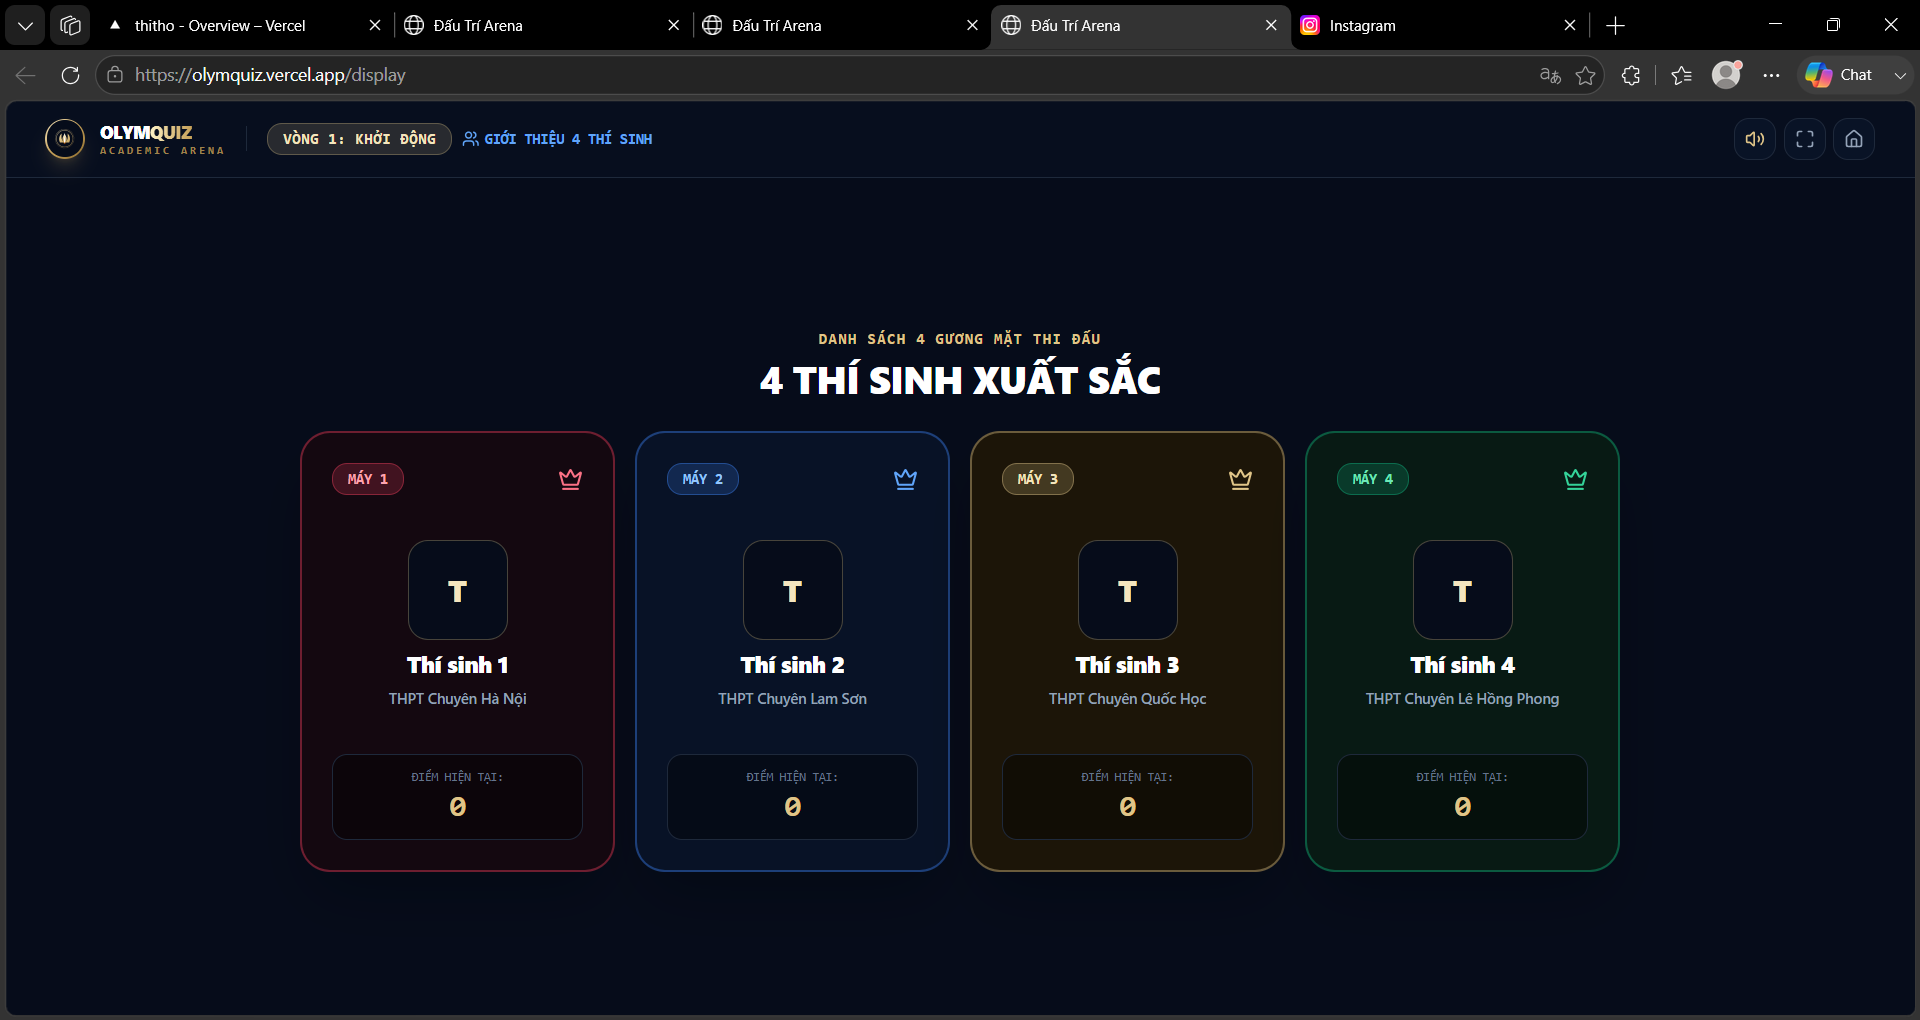
\includegraphics[width=0.95\textwidth]{screenshots/04_display_intro.png}
\end{center}

\vspace{0.4cm}

% ============================================================
% MAN HINH 6: SLIDE THE LE TONG QUAN 4 VONG
% ============================================================
\noindent{\Large\bfseries\color{primary} MAN HINH 6: SLIDE THE LE TONG QUAN 4 VONG DAU}\\[0.1cm]
\noindent\textit{Man hinh May Chieu Hoi Truong (\texttt{/display})}\\[0.2cm]
\textbf{Muc dich}: Giup MC pho bien format thi dau tong the cho toan bo khan phong.
\begin{itemize}[leftmargin=*,noitemsep]
    \item Hien thi 4 the the le tom tat: \textbf{Khoi Dong} (15s/cau, +10d) $\rightarrow$ \textbf{VCNV} (4 hang ngang, tu khoa chinh) $\rightarrow$ \textbf{Tang Toc} (10s-20s-30s-40s) $\rightarrow$ \textbf{Ve Dich} (Goi cau hoi, Sao hy vong, Cuop diem).
\end{itemize}

\begin{center}
    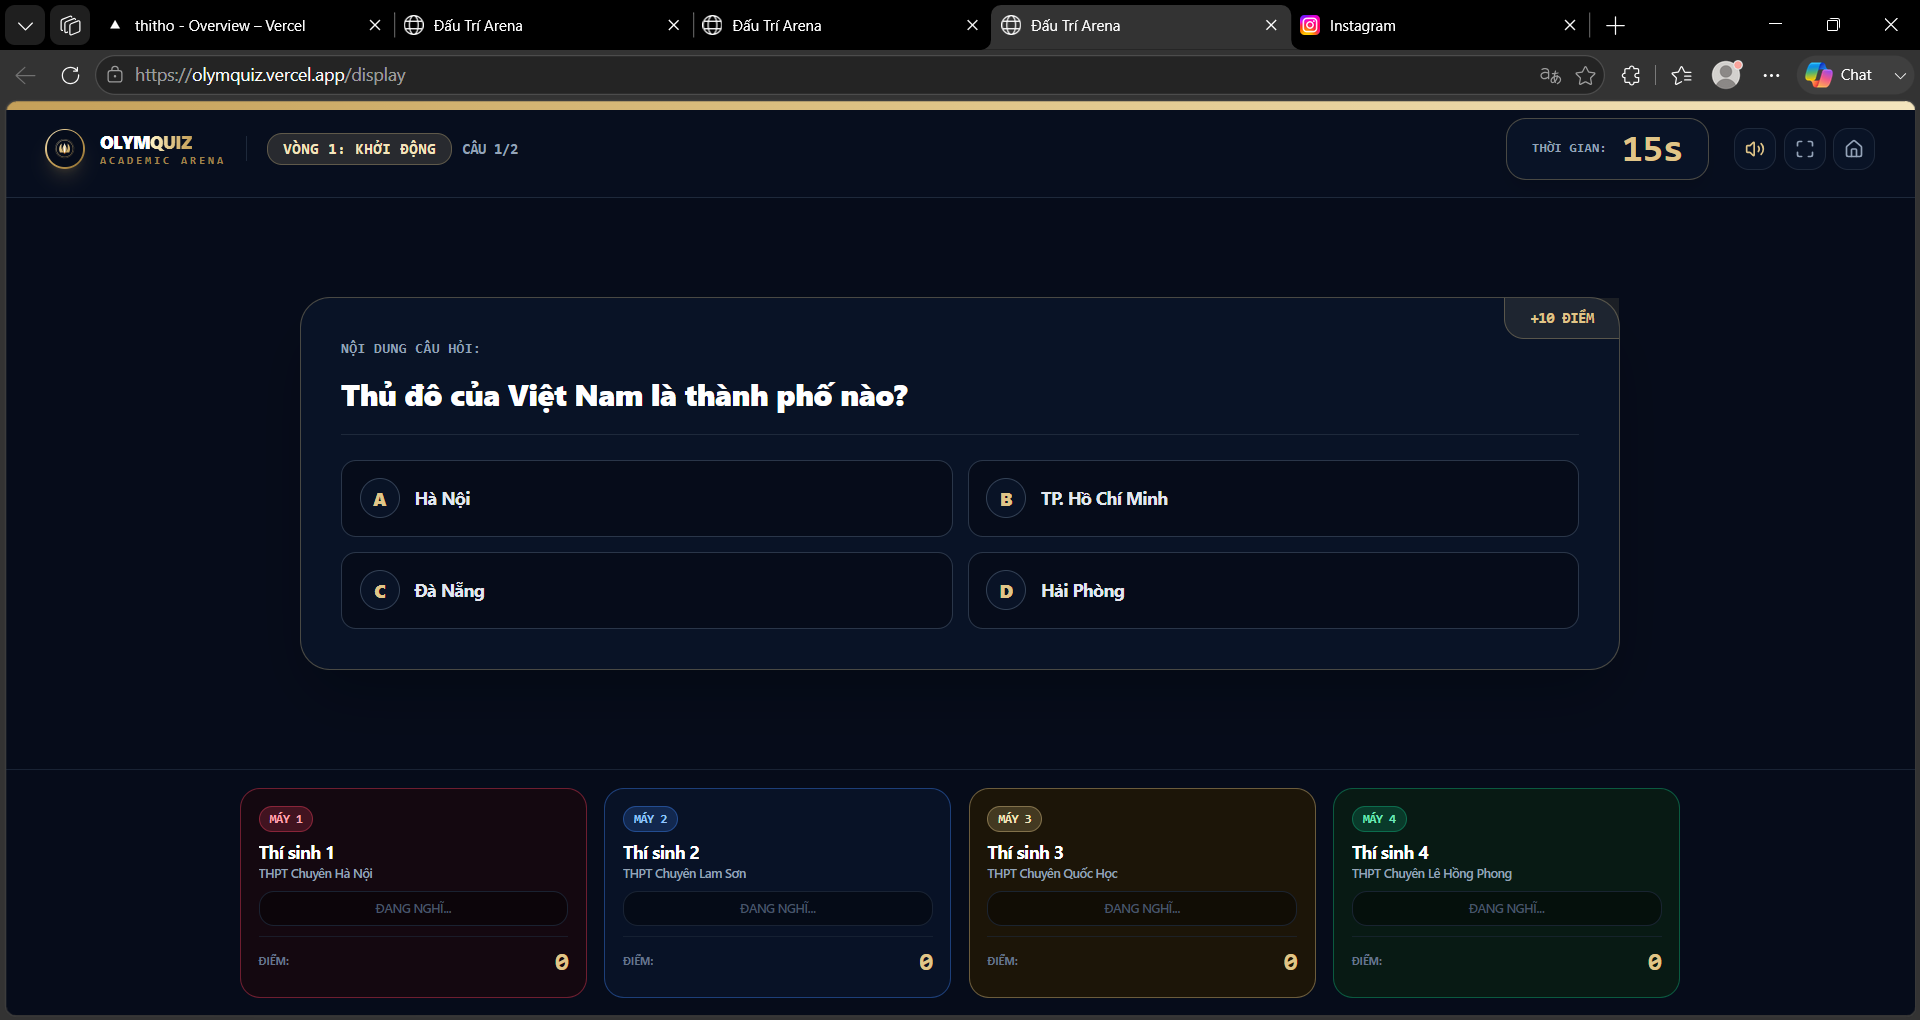
\includegraphics[width=0.95\textwidth]{screenshots/05_display_rules_all.png}
\end{center}

\newpage

% ============================================================
% MAN HINH 7: SLIDE THE LE VONG 1
% ============================================================
\noindent{\Large\bfseries\color{primary} MAN HINH 7: SLIDE CHI TIET THE LE VONG 1 (KHOI DONG)}\\[0.1cm]
\noindent\textit{Man hinh May Chieu Hoi Truong (\texttt{/display})}\\[0.2cm]
\textbf{Muc dich}: Chieu the le chi tiet cua Vong 1 truoc khi bat dau cau hoi dau tien.
\begin{itemize}[leftmargin=*,noitemsep]
    \item Thoi gian lam bai: 15 giay / cau hoi trac nghiem 4 phuong an A, B, C, D.
    \item Co che tinh diem: Tra loi dung duoc +10 Diem. Tra loi sai khong bi tru diem.
\end{itemize}

\begin{center}
    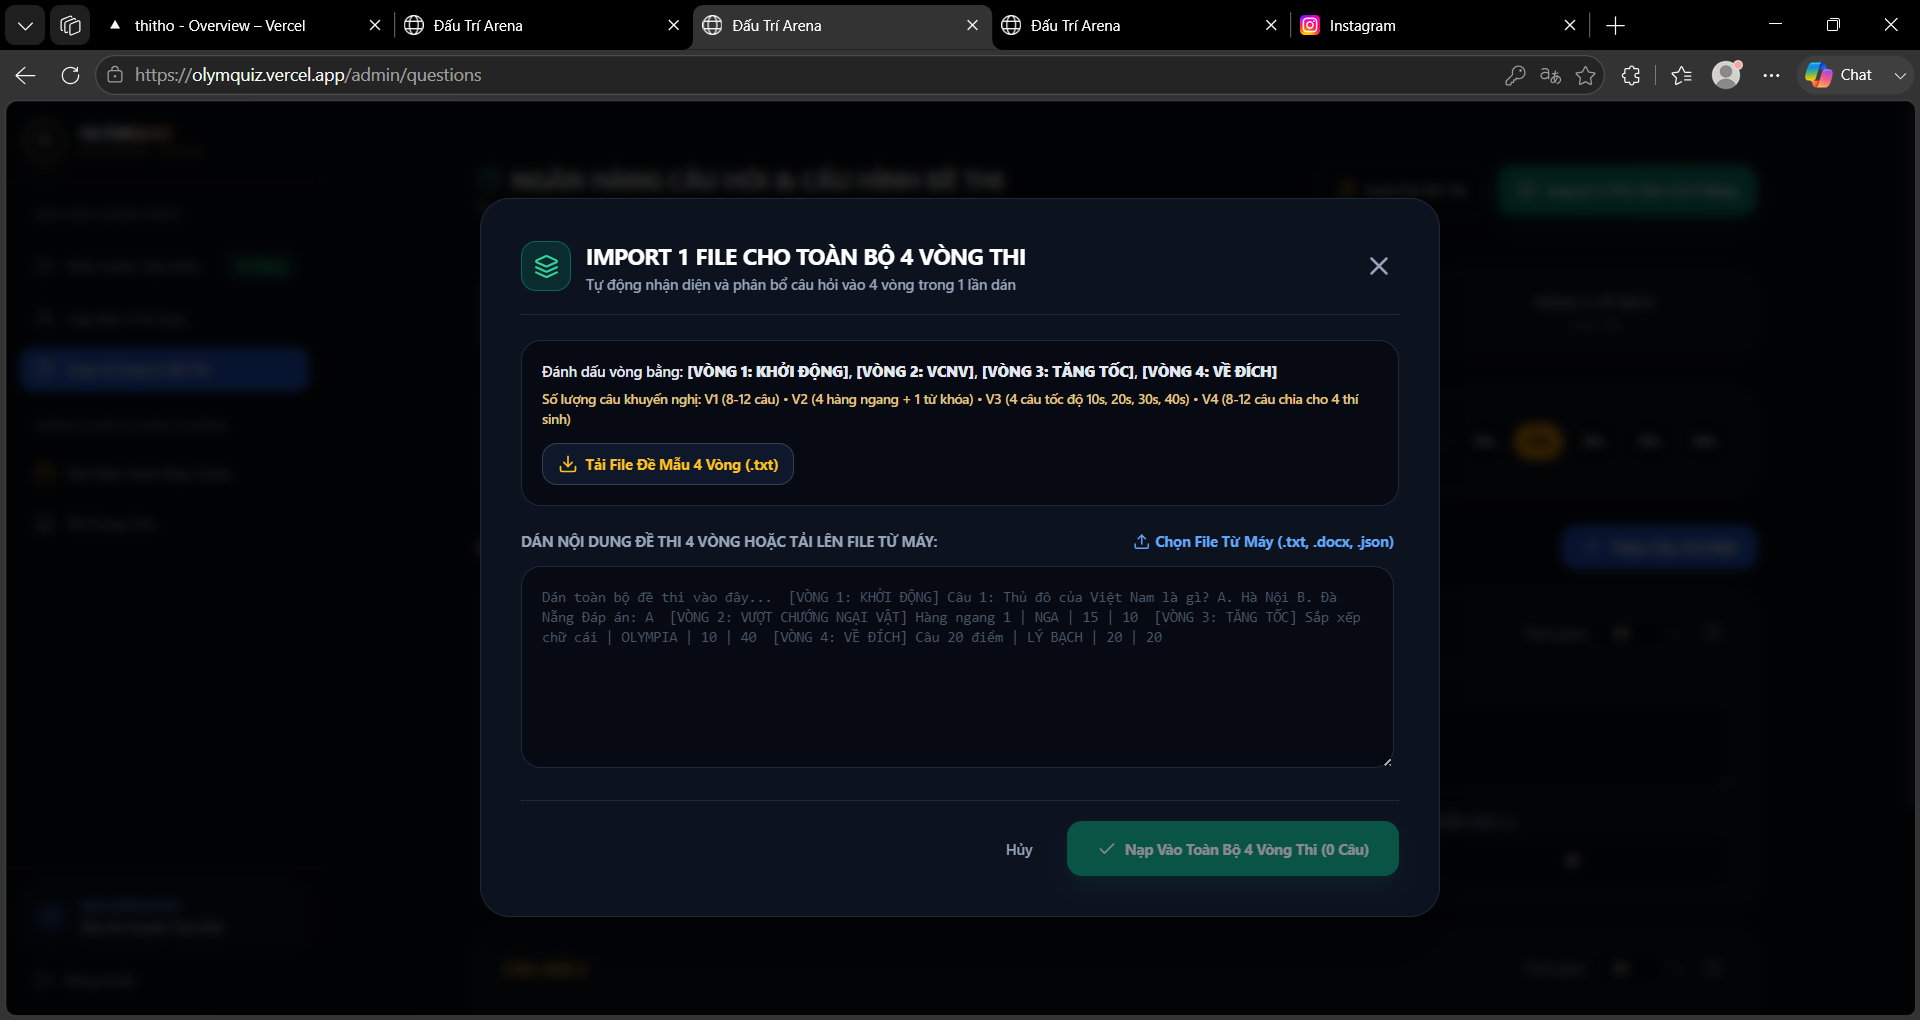
\includegraphics[width=0.95\textwidth]{screenshots/06_display_rule_r1.png}
\end{center}

\vspace{0.4cm}

% ============================================================
% MAN HINH 8: SLIDE THE LE VONG 2
% ============================================================
\noindent{\Large\bfseries\color{primary} MAN HINH 8: SLIDE CHI TIET THE LE VONG 2 (VUOT CHUONG NGAI VAT)}\\[0.1cm]
\noindent\textit{Man hinh May Chieu Hoi Truong (\texttt{/display})}\\[0.2cm]
\textbf{Muc dich}: Chieu luat giai ma 4 hang ngang va quy dinh bam chuong tra loi tu khoa chinh.
\begin{itemize}[leftmargin=*,noitemsep]
    \item Moi cau hang ngang dung duoc +10 Diem kem goi y so luong chu cai.
    \item Bam chuong tra loi Chuong ngai vat: +60d (sau hang 1), +40d (sau hang 2), +20d (sau hang 3). Tra loi sai bi loai khoi vong.
\end{itemize}

\begin{center}
    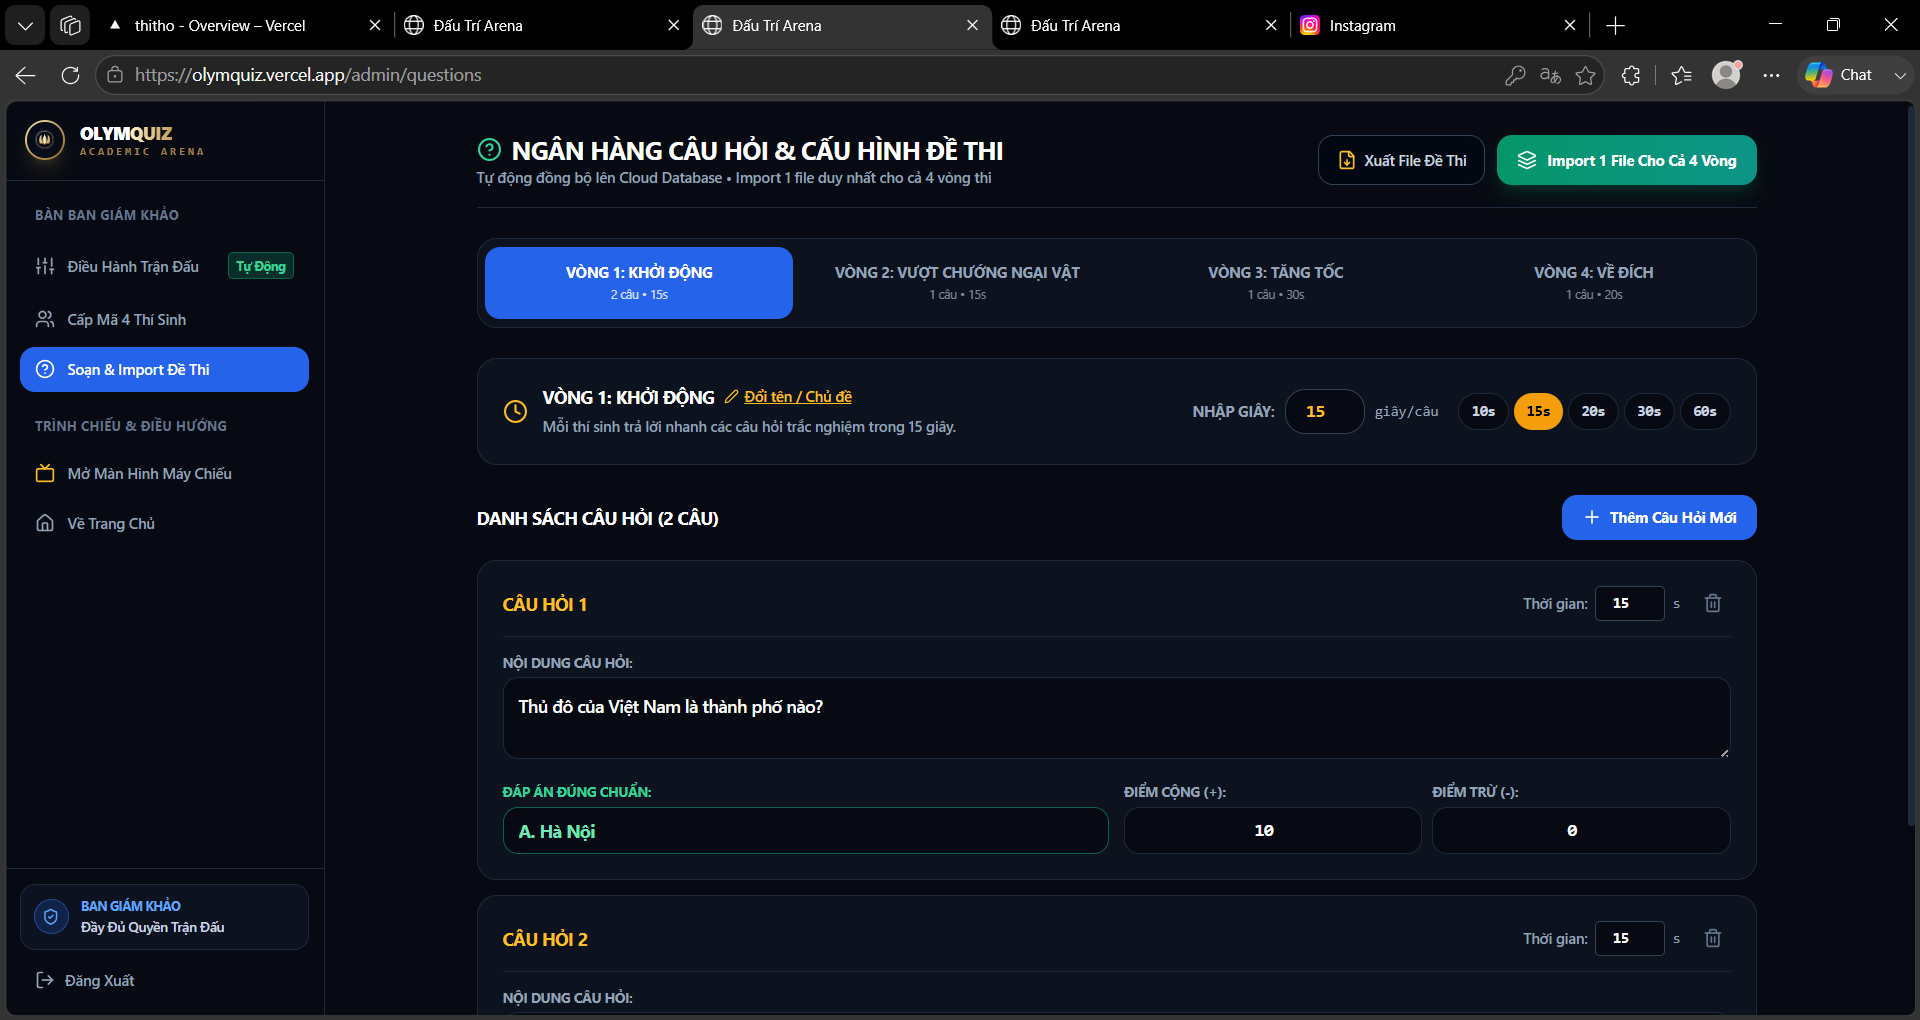
\includegraphics[width=0.95\textwidth]{screenshots/07_display_rule_r2.png}
\end{center}

\newpage

% ============================================================
% MAN HINH 9: SLIDE THE LE VONG 3
% ============================================================
\noindent{\Large\bfseries\color{primary} MAN HINH 9: SLIDE CHI TIET THE LE VONG 3 (TANG TOC)}\\[0.1cm]
\noindent\textit{Man hinh May Chieu Hoi Truong (\texttt{/display})}\\[0.2cm]
\textbf{Muc dich}: Chieu luat cuoc dua toc do tinh bang mili-giay.
\begin{itemize}[leftmargin=*,noitemsep]
    \item 4 moc thoi gian tang dan: 10 giay (cau 1) $\rightarrow$ 20 giay (cau 2) $\rightarrow$ 30 giay (cau 3) $\rightarrow$ 40 giay (cau 4).
    \item Thang diem cong theo toc do nop: Nhanh nhat (+40d) $\rightarrow$ Nhi (+30d) $\rightarrow$ Ba (+20d) $\rightarrow$ Tu (+10d).
\end{itemize}

\begin{center}
    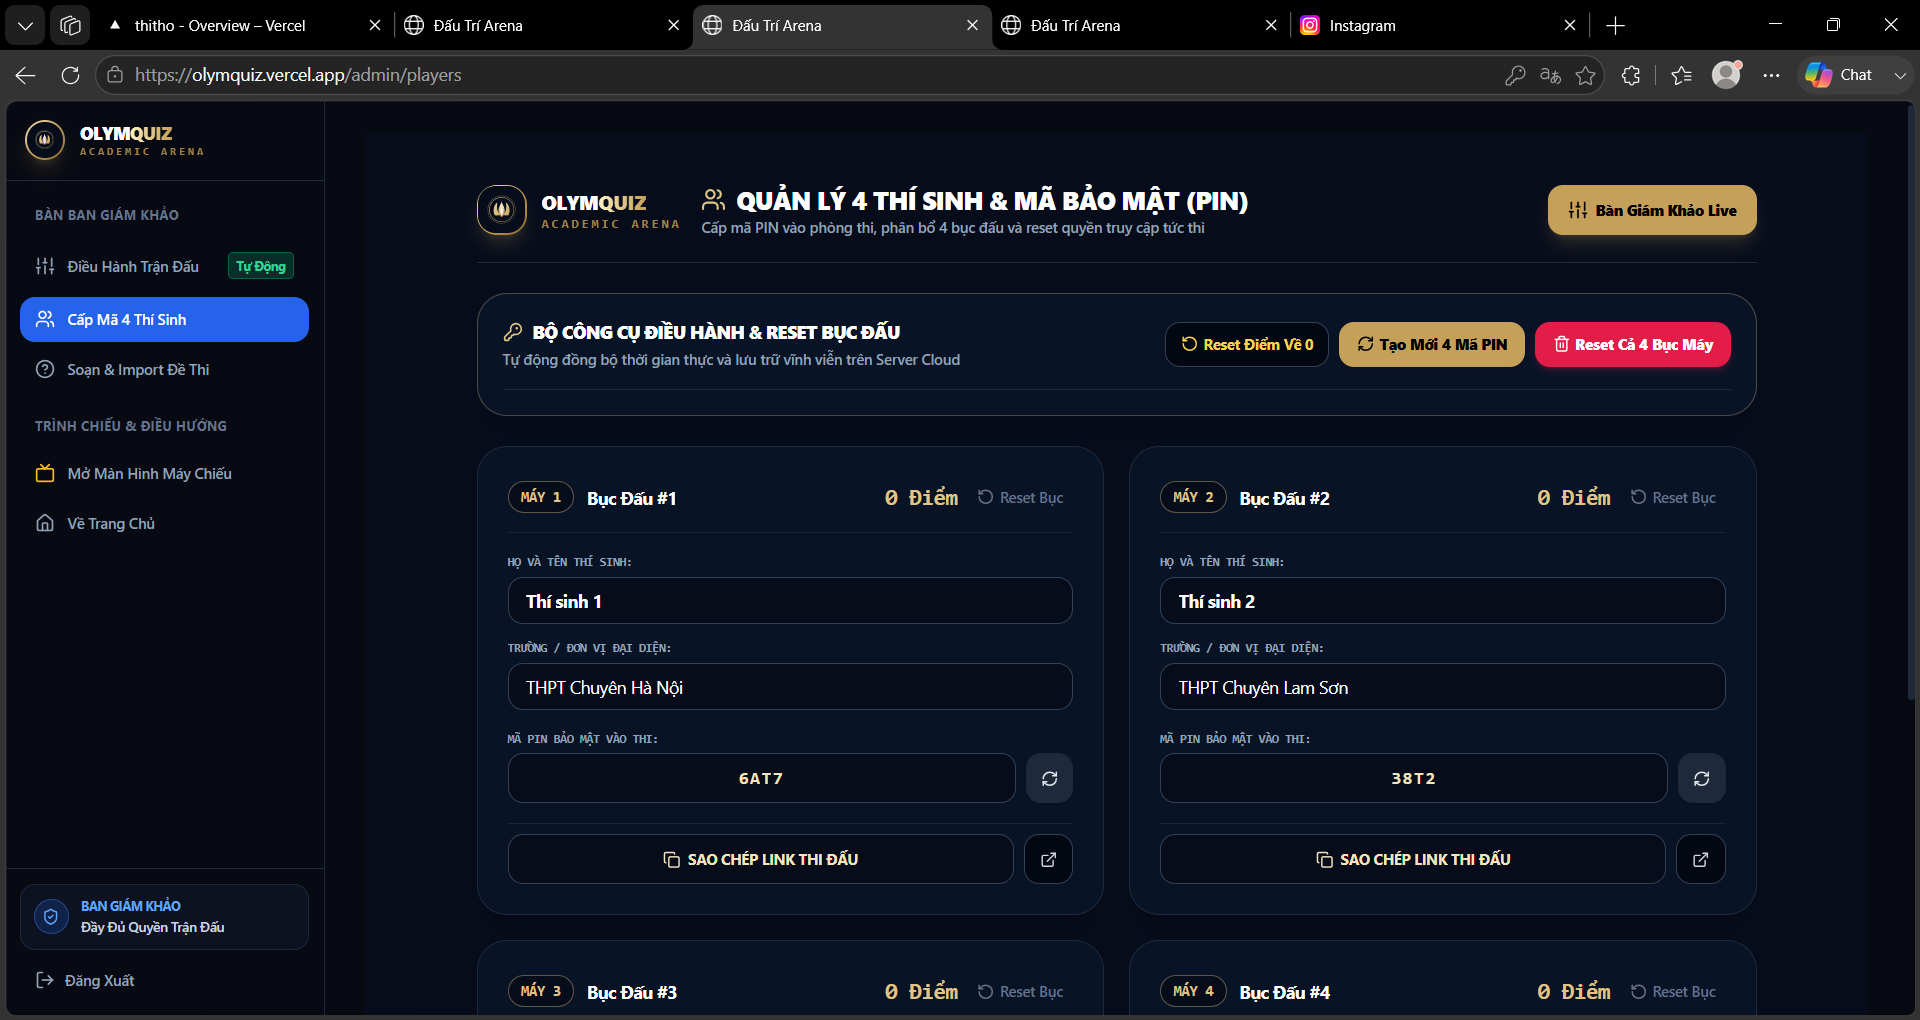
\includegraphics[width=0.95\textwidth]{screenshots/08_display_rule_r3.png}
\end{center}

\vspace{0.4cm}

% ============================================================
% MAN HINH 10: SLIDE THE LE VONG 4
% ============================================================
\noindent{\Large\bfseries\color{primary} MAN HINH 10: SLIDE CHI TIET THE LE VONG 4 (VE DICH)}\\[0.1cm]
\noindent\textit{Man hinh May Chieu Hoi Truong (\texttt{/display})}\\[0.2cm]
\textbf{Muc dich}: Chieu luat goi cau hoi 20d/30d, Ngoi Sao Hy Vong va Chuong cuop diem.
\begin{itemize}[leftmargin=*,noitemsep]
    \item Moi ban co 1 luot thi chinh. Duoc quyen dat \textbf{Ngoi Sao Hy Vong} (+x2 diem neu dung, -50\% neu sai).
    \item Neu thi sinh chinh tra loi sai, 3 ban con lai duoc quyen Bam Chuong Cuop Diem.
\end{itemize}

\begin{center}
    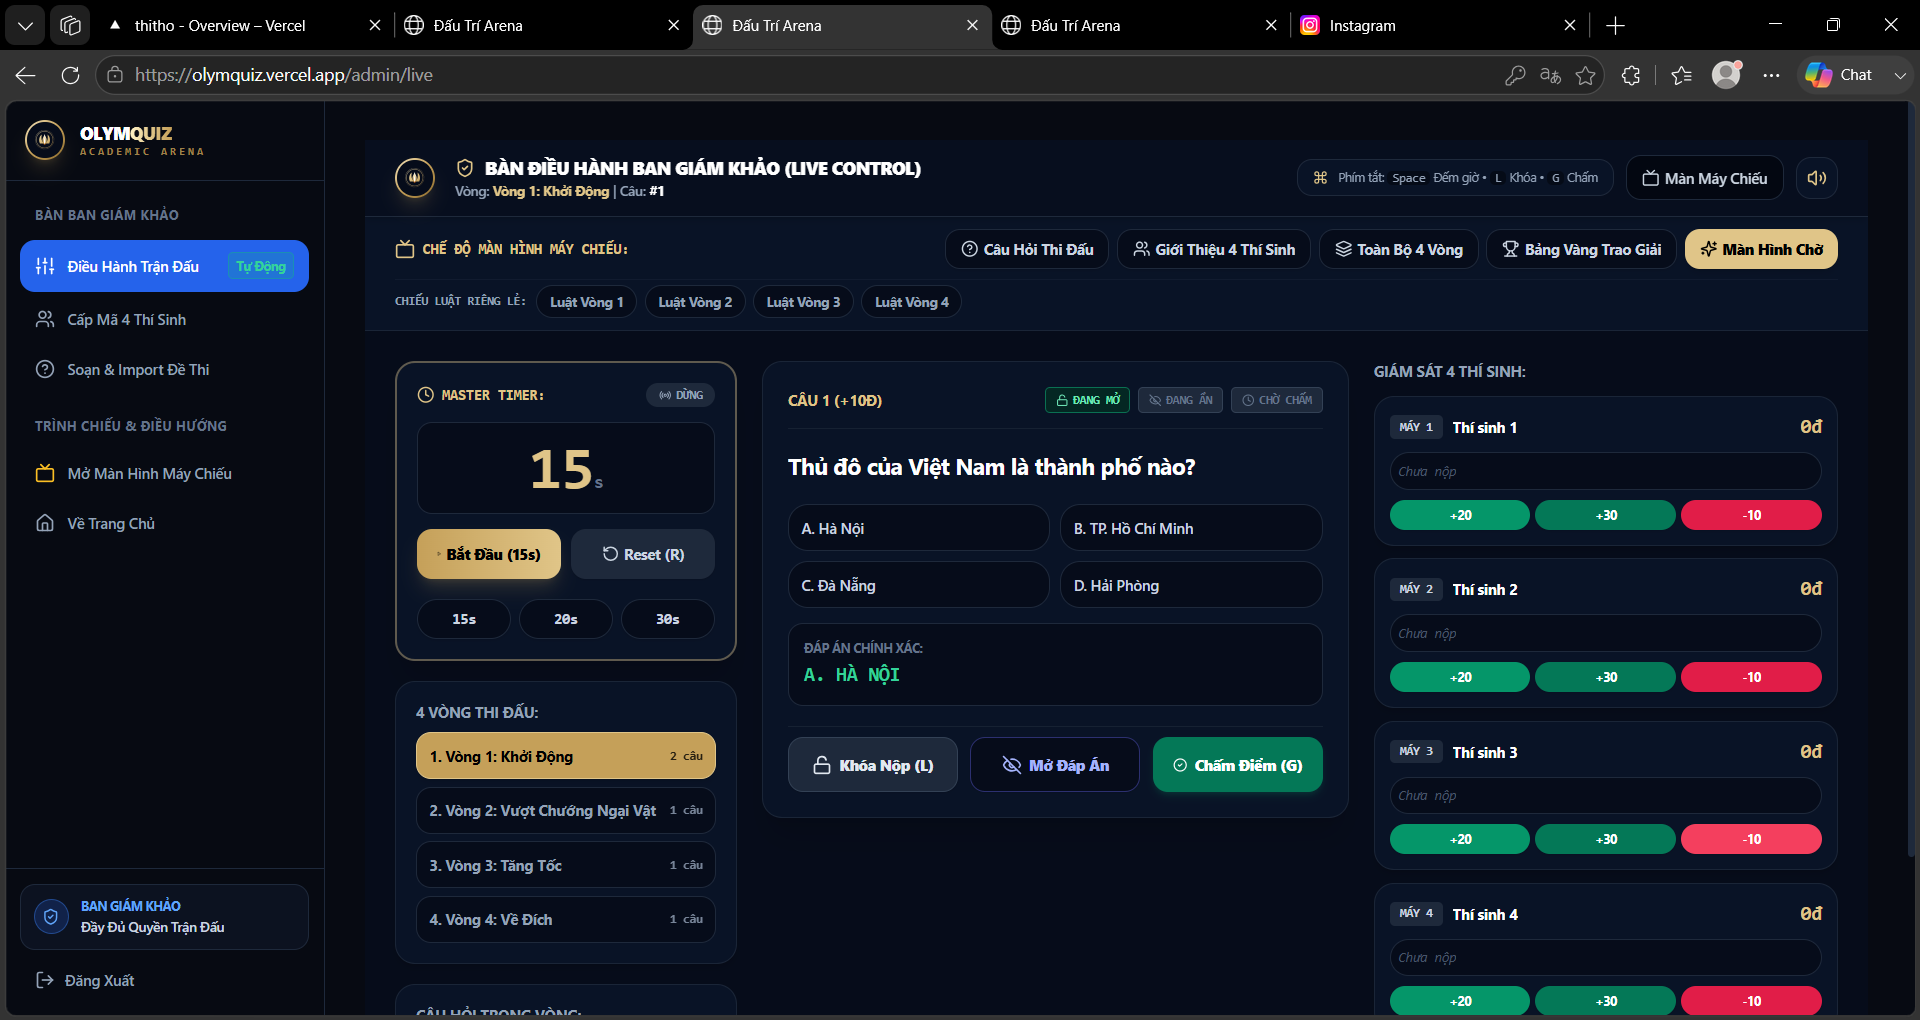
\includegraphics[width=0.95\textwidth]{screenshots/09_display_rule_r4.png}
\end{center}

\newpage

% ============================================================
% MAN HINH 11: MAY CHIEU THI DAU CAU 1
% ============================================================
\noindent{\Large\bfseries\color{primary} MAN HINH 11: MAN MAY CHIEU CAU HOI 1 (DA CONG BO DAP AN)}\\[0.1cm]
\noindent\textit{Man hinh May Chieu Hoi Truong (\texttt{/display})}\\[0.2cm]
\textbf{Muc dich}: Hien thi ket qua cong khai va minh bach cho toan bo khan phong.
\begin{itemize}[leftmargin=*,noitemsep]
    \item \textbf{Phuong An Dung (Ha Noi)}: Tu dong phat sang vien xanh ngoc bich noi bat.
    \item \textbf{4 Buc Diem Duoi Chan}: Tu dong hien dap an cua tung ban kem dau tick xanh cho cau dung va dau nhan do cho cau sai.
\end{itemize}

\begin{center}
    
\includegraphics[width=0.95\textwidth]{screenshots/02_display_q1.png}
\end{center}

\vspace{0.4cm}

% ============================================================
% MAN HINH 12: MAY CHIEU THI DAU CAU 2
% ============================================================
\noindent{\Large\bfseries\color{primary} MAN HINH 12: MAN MAY CHIEU CAU HOI 2 (DANG DEM LUI THOI GIAN)}\\[0.1cm]
\noindent\textit{Man hinh May Chieu Hoi Truong (\texttt{/display})}\\[0.2cm]
\textbf{Muc dich}: Giao dien thi dau truc tiep khi dong ho dang chay.
\begin{itemize}[leftmargin=*,noitemsep]
    \item \textbf{Thanh Laser Timer tren cung}: Chay lui theo thoi gian thuc (doi mau do khi con duoi 3 giay).
    \item \textbf{Dong ho LED to}: Hien thi so giay con lai sac net o goc phai tren.
\end{itemize}

\begin{center}
    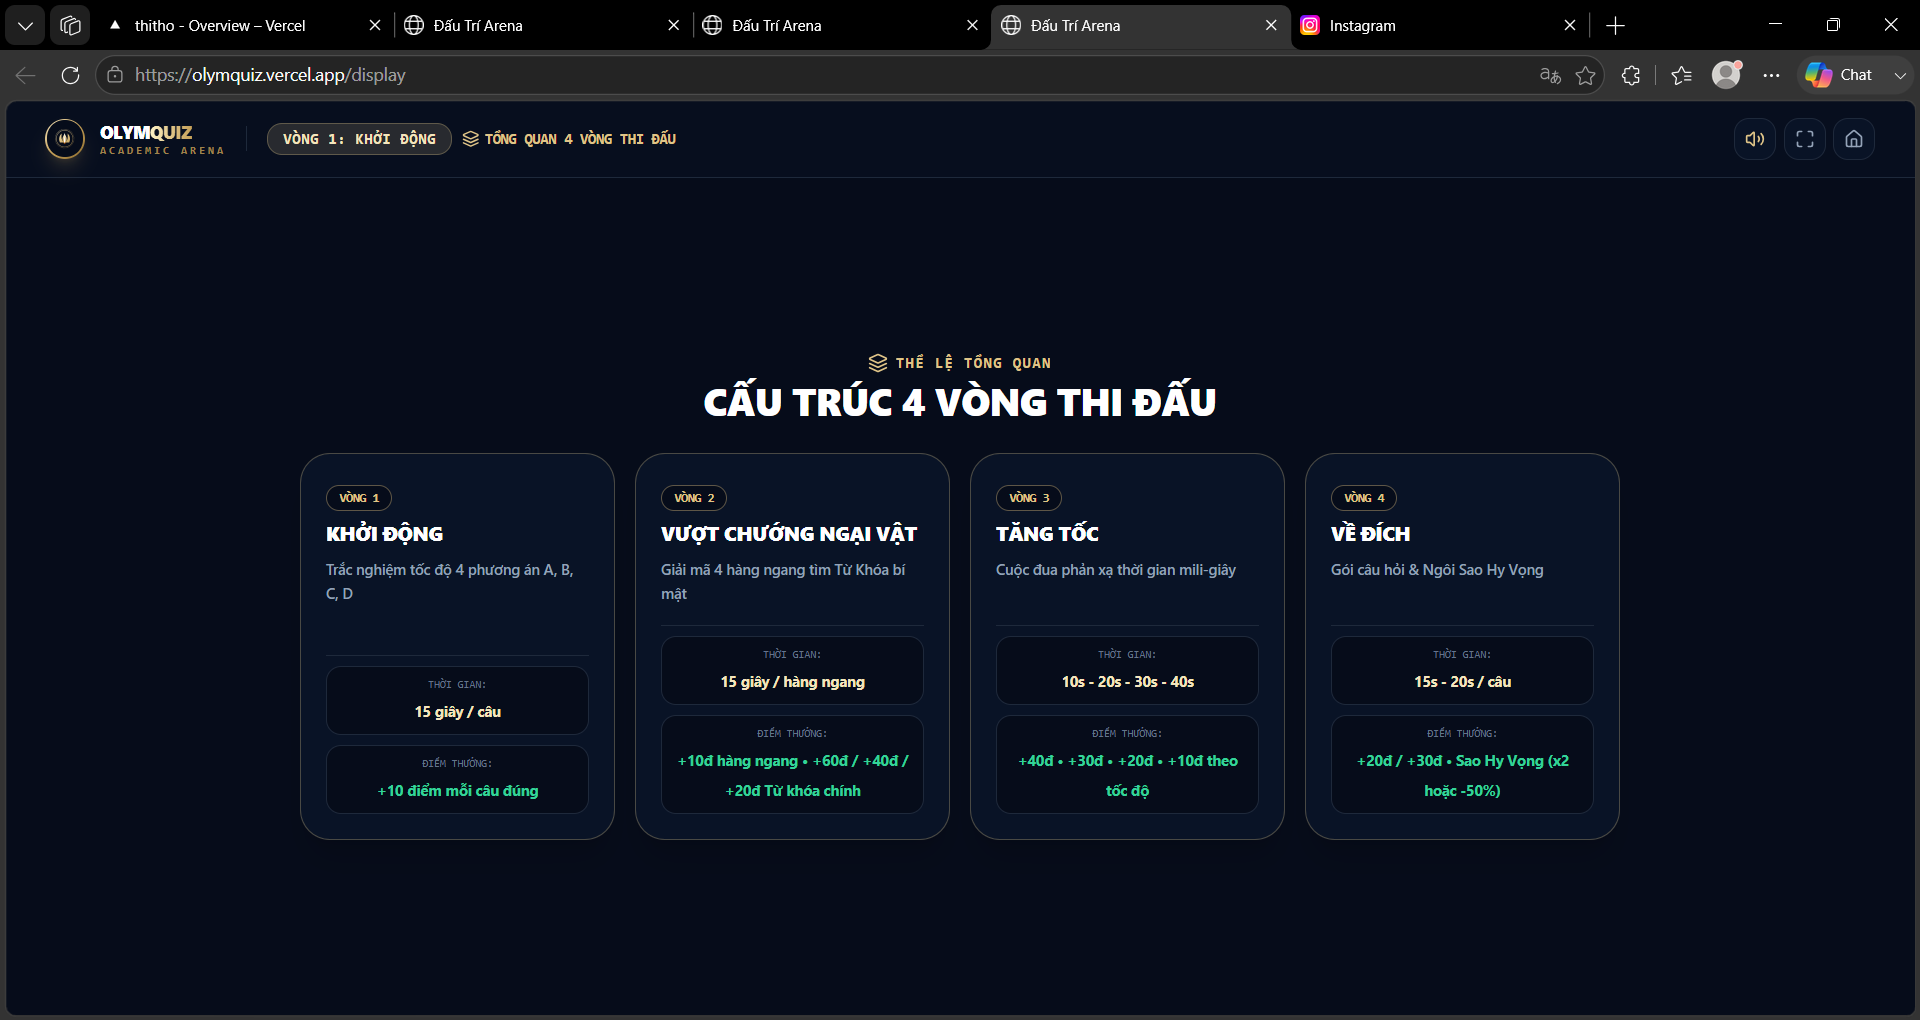
\includegraphics[width=0.95\textwidth]{screenshots/03_display_q2.png}
\end{center}

\newpage

% ============================================================
% MAN HINH 13: BANG VANG TRAO GIAI
% ============================================================
\noindent{\Large\bfseries\color{primary} MAN HINH 13: SLIDE BANG VANG VINH DANH VA TRAO GIAI}\\[0.1cm]
\noindent\textit{Man hinh May Chieu Hoi Truong (\texttt{/display})}\\[0.2cm]
\textbf{Muc dich}: Man hinh be mac vinh danh nha vo dich va trao giai.
\begin{itemize}[leftmargin=*,noitemsep]
    \item He thong tu dong xep thu hang \textbf{Quan Quan - A Quan - Hang Ba - Hang Tu} dua tren tong diem.
    \item Tu dong kich hoat hieu ung \textbf{Phao Hoa Confetti ruc ro} va bieu tuong Vuong mien Hoang kim!
\end{itemize}

\begin{center}
    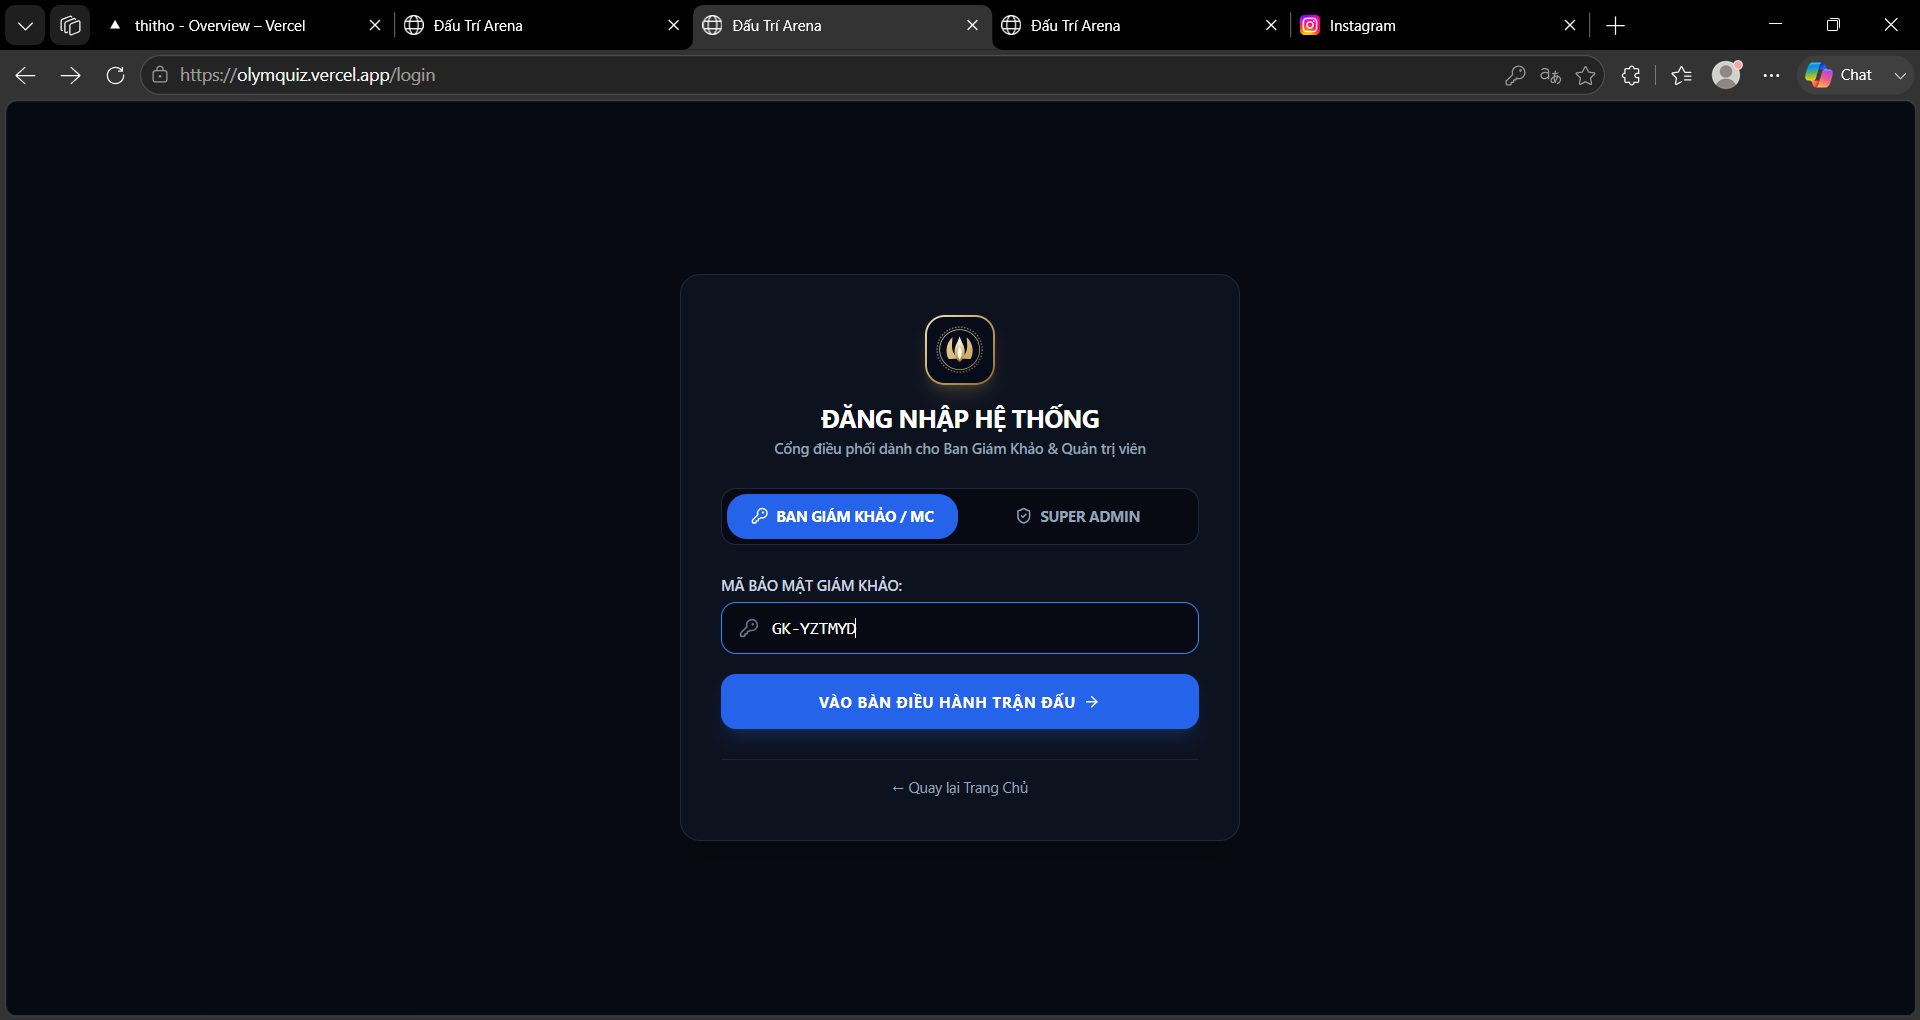
\includegraphics[width=0.95\textwidth]{screenshots/10_display_leaderboard.png}
\end{center}

\vspace{0.8cm}
\begin{center}
    \rule{\textwidth}{1.5pt}\\[0.3cm]
    {\Large\bfseries\color{primary} CHUC BAN VA NGUOI YEU TO CHUC BUOI THI DAU THANH CONG RUC RO!}\\[0.2cm]
    {\small Ban quyen 2026 OlymQuiz Academic Arena -- Website truc tuyen: \texttt{https://olymquiz.vercel.app}}
\end{center}

\end{document}
